模拟数据和数字数据都可以转换为模拟信号或数字信号。\textbf{将模拟数据或数字数据(可统称为数据)转换为模拟信号的过程称为调制};\textbf{将模拟数据或数字数据转换为数字信号的过程称为编码},如图2-3所示。

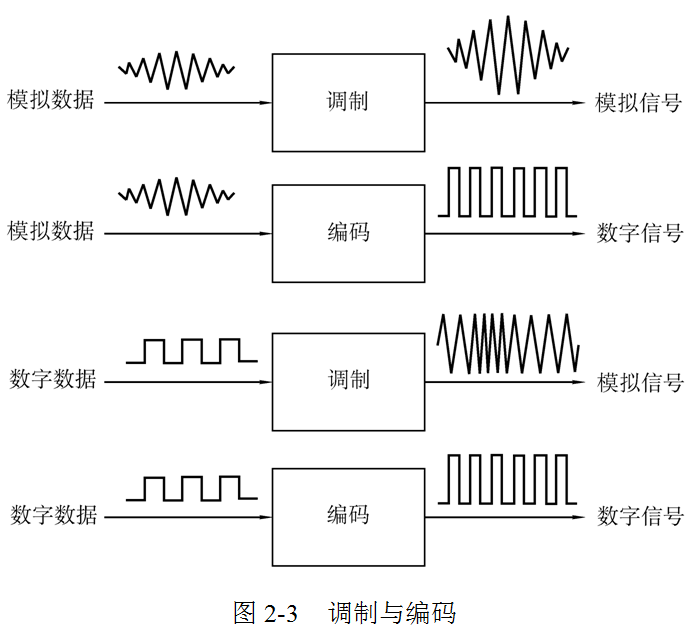
\includegraphics[width=3.43750in,height=3.09375in]{png-jpeg-pics/EB621C2074FA45D90973D4B8CA7D451F.png}

\textbf{{调制}}

\textbf{{一、数字数据调制为模拟信号}}

数字数据调制技术\textbf{在发送端将数字信号转换为模拟信号},而\textbf{在接收端将模拟信号还原为数字信号},分别对应于调制解调器的调制和解调过程。考研中理解这两种转换即可,其他的了解即可。

{\textbf{故事助记:}调制解调器的调制是为了将数字数据转换成模拟信号,因为数字数据含有太多的低频成分(可以看成矮个子),而该信道不让他过去的原因有两种:}\\
{\textbf{原因一:}太矮了(都是低频成分),不让他过去。}\\
{\textbf{原因二:}他穿的衣服不适合该场合(低频成分不能与信道的特性相适应)。}\\
{针对以上两种原因,可以想出两种办法。}\\
{针对第一种原因:让他变高。}\\
{针对第二种原因:换件正式的西装。}{}

\textbf{这样就引入了两种调制,如下:}\\
1.
带通调制(把矮个子变高):类似于增高垫,让矮个子变高了,这样就可以过去了,即教材所讲的将基带信号的频率范围搬移到较高的频段以便在信道中传输由此引出了3种方式:调幅、调频和调相。\\
2.
基带调制(换件西装):给基带信号的低频成分改变波形,使之适应信道的特性(也就是说给矮个子穿上西装,改变一下外表,使之适应这个场合);但是穿上西装仍然是矮子,也就是说基带信号的低频成分改变波形仍然是基带信号,没有变成其他信号。

\textbf{{二、模拟数据调制为模拟信号}}\\
模拟数据调制为模拟信号主要有以下原因:\\
1. 为了实现传输的有效性,可能需要较高的频率。\\
2. 充分利用带宽。

\textbf{{编码}}

\textbf{{一、数字数据编码为数字信号}}

数字数据编码用于基带信号传输中,可以在基本不改变数字数据信号频率的情况下,直接传输数字信号,即直接让矮子过去,不用穿增高垫了。既然不用穿增高垫,那就必须穿西装过去,而现在西装又分很多种牌子(非归零码、曼彻斯特编码、差分曼彻斯特编码)。

1.~\textbf{非归零码:}用低电平表示0,高电平表示1;或者反过来。缺点是无法判断一个码元的开始和结束,收发双方难以保持同步。

2.~\textbf{曼彻斯特编码:}将每个码元分成两个相等的间隔。前一个间隔为高电平而后一个间隔为低电平表示码元1;码元0正好相反。曼彻斯特编码的特点是将每个码元的中间跳变作为收发双方的同步信号,无需额外的同步信号;\textbf{但它所占的频带宽度是原始的基带宽度的两倍}。

3.~\textbf{差分曼彻斯特编码:}若码元为1,则其前半个码元的电平与上一个码元的后半个码元的电平一样;若码元为0,则其前半个码元的电平与上一个码元的后半个码元的电平相反。在每个码元的中间,都有一次电平的跳转。该编码技术较复杂,但抗干扰性较好。

\textbf{{二、}{模拟数据编码为数字信号}}

此编码最典型的例子就是\textbf{脉冲编码调制}。

\textbf{脉冲编码调制:}只需记住3个步骤,\textbf{采样、量化和编码}以及它是将模拟数据进行数字信号编码即可。
